% This section should reintroduce the full data flow diagram from the architectural specification, and discuss at a high level the purpose of each layer. You do not need to include a subsection for each layer, a 1 - 2 paragraph recap is sufficient.
\begin{flushleft}
The system for our product is currently simplified into 4 layers and 3 high-level components. Each layer/component will interact with one another in different ways.
\end{flushleft}
\begin{flushleft}
The Opponent is the person that will be going against the robot during the checkers game. The Input Device is one of the ways the opponent will be able to facilitate the progression of the checkers match. The camera is the component that acts as the eyes into the real world for our system. The Move Decision layer is the layer that will make all of the move decisions that the robot will make. This layer consists of Computer Vision and AI. The Computer layer is the central piece of our system. This layer acts as the facilitator of the checkers match, and receives input from the Opponent to progress the match, sends signals to the AI layer to grab board state and make a move, and signals the UR5 Robot Arm layer to execute those moves. The Move Execution layer is the layer that will physically execute the moves that our system will make during a checkers match with the robot arm and related parts. And finally, The External Components layer is composed of all of the physical checkers board game pieces. Both the Opponent component and the Move Execution layer physically interact with the External Components layer when they have made their move decisions to progress the match.
\end{flushleft}

\begin{figure}[h!]
	\centering
 	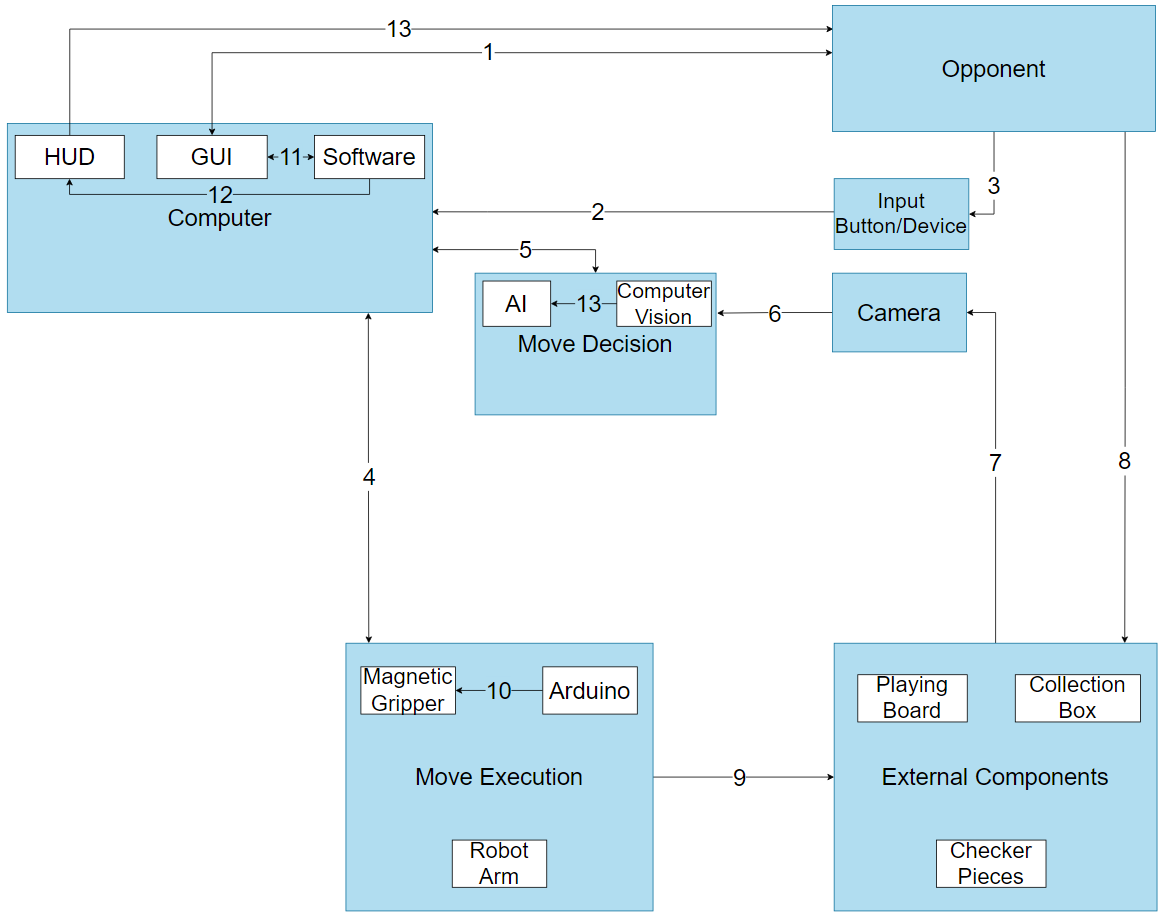
\includegraphics[width=0.90\textwidth]{images/data_flow_actual}
 \caption{System architecture}
\end{figure}
